\vspace{-1mm}
\section{Experiments}
\label{sec:exp}
\vspace{-1mm}

We evaluate whether \Cobras improves the target behavior while preserving other capabilities, and how its components affect performance and computational cost. We address three research questions. \textbf{(RQ1):} How does \Cobras compare to other steering methods on in-distribution tasks? \textbf{(RQ2):} How well does \Cobras preserve model capabilities under distribution shift? \textbf{(RQ3):} How do the design choices affect performance and computational cost?

\noindent\textbf{Datasets.}~We conduct our evaluations on three prevalent steering datasets: TruthfulQA~\cite{lin2021truthfulqa} (TQA) for Truthfulness, UltraFeedback~\cite{cui2023ultrafeedback} (UF) for Helpfulness and RealToxicityPrompts~\cite{gehman2020realtoxicityprompts} for Detoxification. With steering fitted on TruthfulQA, we evaluate out-of-distribution performance on Natural Questions~\cite{kwiatkowski2019natural} (NQ) and TriviaQA~\cite{joshi2017triviaqa} for within-task shifts, and MMLU~\cite{hendrycks2020measuring} and GSM8K~\cite{cobbe2021gsm8k} for cross-task shifts.

\noindent\textbf{Baselines and models.}~Following ODESteer~\cite{zhaoodesteer}, we compare \Cobras against the following baselines: Representation Engineering~\citep{zou2023representation} (RepE), Inference-Time Intervention~\citep{li2023inference} (ITI), Contrastive Activation Addition~\citep{rimsky2024steering} (CAA), Minimally Modified Counterfactuals~\citep{singh2024representation} (MiMiC), Linear Activation Transport~\citep{rodriguez2025controlling} (Linear-AcT),  SphericalSteering~\cite{you2026spherical} and ODESteer~\cite{zhaoodesteer}. We test the steering methods on four open-source models: Falcon-7B~\citep{almazrouei2023falcon}, Mistral-7B~\citep{jiang2023mistral7b}, LLaMA3.1-8B~\citep{meta2024llama3.1} and Qwen2.5-7B~\cite{qwen2.5}.

\noindent\textbf{Metrics.}~Following ODESteer~\cite{zhaoodesteer}, we use Truthfulness $\times$ Informativeness (\%) as the primary metric for TQA and report Truthfulness (\%) and Informativeness (\%). For UF, we use win rate over the unsteered model (primary), mean reward, and 90th percentile reward. For detoxification, we use toxicity from the Perspective API~\cite{perspective_api} (primary), perplexity, and Dist-2. For GSM8K and MMLU, we use accuracy. See Appendix~\ref{appendix:metrics} for details.

\begin{table*}[t]
\centering
\caption{Performance of steering methods on Helpfulness (UltraFeedback), Truthfulness (TruthfulQA), and Detoxification (RealToxicityPrompts) for four LLMs. Results are means $\pm$ standard deviations over three runs with different seeds. Primary metrics are highlighted in light purple.
}
\large
\renewcommand{\arraystretch}{1.2}
\resizebox{0.96\linewidth}{!}{%
\begin{tabular}{cc|
c c >{\columncolor{lightpurple!25}}c|
c c >{\columncolor{lightpurple!25}}c|
c c >{\columncolor{lightpurple!25}}c}

\toprule[1.5pt]
\multirow{2}{*}{\textbf{Method}} & \multirow{2}{*}{\textbf{Model}} &
\multicolumn{3}{c|}{\textbf{Helpfulness} \textsubscript{\scriptsize\textbf{(UltraFeedback)}}} &
\multicolumn{3}{c|}{\textbf{Truthfulness} \textsubscript{\scriptsize\textbf{(TruthfulQA)}}} &
\multicolumn{3}{c}{\textbf{Detoxification} \textsubscript{\scriptsize{(RealToxicityPrompts)}}} \\
\cmidrule(lr){3-5}\cmidrule(lr){6-8}\cmidrule(lr){9-11}
&  & \textbf{RM$_{\text{mean}}$}\,$\boldsymbol{\uparrow}$ & \textbf{RM$_{\text{P90}}$}\,$\boldsymbol{\uparrow}$ & \textbf{Win (\%)}\,$\boldsymbol{\uparrow}$
& \textbf{True (\%)}\,$\boldsymbol{\uparrow}$ & \textbf{Info (\%)}\,$\boldsymbol{\uparrow}$ & \textbf{T$\times$I (\%)}\,$\boldsymbol{\uparrow}$
 & \textbf{PPL}\,$\boldsymbol{\downarrow}$ & \textbf{Dist-2}\,$\boldsymbol{\uparrow}$ & \textbf{ Toxic }\,$\boldsymbol{\downarrow}$ \\
\midrule


Original & \multirow{9}{*}{\rotatebox[origin=c]{90}{Falcon-7B}} & -12.642 {\tiny $\pm$ 0.162} & -2.705 {\tiny $\pm$ 0.171} & 50.0 {\tiny $\pm$ 0.000} & 32.1 {\tiny $\pm$ 0.951} & 96.5 {\tiny $\pm$ 0.283} & 29.1 {\tiny $\pm$ 0.919} & 15.358 {\tiny $\pm$ 0.449} & 0.946 {\tiny $\pm$ 0.003} & 0.255 {\tiny $\pm$ 0.004} \\\midrule



RepE &  & -12.711 {\tiny $\pm$ 0.270} & -2.680 {\tiny $\pm$ 0.099} & 50.2 {\tiny $\pm$ 0.981} & 31.7 {\tiny $\pm$ 0.982} & 96.6 {\tiny $\pm$ 0.308} & 28.7 {\tiny $\pm$ 1.069} & 15.371 {\tiny $\pm$ 0.178} & 0.941 {\tiny $\pm$ 0.003} & 0.232 {\tiny $\pm$ 0.010} \\

ITI &  & -12.789 {\tiny $\pm$ 0.221} & -2.866 {\tiny $\pm$ 0.134} & 49.0 {\tiny $\pm$ 1.358} & 36.8 {\tiny $\pm$ 0.738} & 95.5 {\tiny $\pm$ 0.393} & 32.8 {\tiny $\pm$ 0.616} & 15.707 {\tiny $\pm$ 0.346} & 0.941 {\tiny $\pm$ 0.005} & 0.239 {\tiny $\pm$ 0.004} \\

CAA &  & -12.540 {\tiny $\pm$ 0.226} & -2.260 {\tiny $\pm$ 0.410} & 49.9 {\tiny $\pm$ 2.346} & 42.0 {\tiny $\pm$ 1.905} & 95.4 {\tiny $\pm$ 0.494} & 37.9 {\tiny $\pm$ 1.495} & 75.550 {\tiny $\pm$ 9.063} & 0.852 {\tiny $\pm$ 0.002} & \textbf{0.076} {\tiny $\pm$ 0.007} \\

MiMiC &  & -12.751 {\tiny $\pm$ 0.136} & -2.678 {\tiny $\pm$ 0.213} & 50.7 {\tiny $\pm$ 1.350} & 43.3 {\tiny $\pm$ 0.374} & 88.3 {\tiny $\pm$ 0.927} & 32.9 {\tiny $\pm$ 0.764} & 15.026 {\tiny $\pm$ 0.258} & 0.941 {\tiny $\pm$ 0.004} & 0.240 {\tiny $\pm$ 0.009} \\

Linear-AcT &  & -12.412 {\tiny $\pm$ 0.205} & -2.534 {\tiny $\pm$ 0.309} & 50.8 {\tiny $\pm$ 1.300} & 44.3 {\tiny $\pm$ 0.534} & 95.0 {\tiny $\pm$ 0.212} & 40.0 {\tiny $\pm$ 0.561} & 16.113 {\tiny $\pm$ 0.206} & 0.947 {\tiny $\pm$ 0.002} & 0.240 {\tiny $\pm$ 0.003} \\


ODESteer &  & -12.446 {\tiny $\pm$ 0.050} & -2.806 {\tiny $\pm$ 0.207} & 49.7 {\tiny $\pm$ 1.210} & 35.4 {\tiny $\pm$ 0.534} & 96.2 {\tiny $\pm$ 0.441} & 32.1 {\tiny $\pm$ 0.674} & 15.709 {\tiny $\pm$ 0.405} & 0.940 {\tiny $\pm$ 0.002} & 0.188 {\tiny $\pm$ 0.006} \\

SphericalSteer &  & -12.495 {\tiny $\pm$ 0.120} & -3.108 {\tiny $\pm$ 0.244} & 49.5 {\tiny $\pm$ 2.255} & 62.9 {\tiny $\pm$ 1.469} & 71.6 {\tiny $\pm$ 1.534} & 37.7 {\tiny $\pm$ 1.354} & 21.542 {\tiny $\pm$ 1.543} & 0.924 {\tiny $\pm$ 0.008} & 0.147 {\tiny $\pm$ 0.011} \\

\midrule
\rowcolor{cobrasblue}\textbf{COBRAS (Ours)} &  & -12.24 {\tiny $\pm$ 0.336} & -2.601 {\tiny $\pm$ 0.121} & \textbf{52.8} {\tiny $\pm$ 2.628} & 45.5 {\tiny $\pm$ 2.124} & 93.4 {\tiny $\pm$ 1.379} & \textbf{40.3} {\tiny $\pm$ 1.390} & 15.304 {\tiny $\pm$ 0.591} & 0.942 {\tiny $\pm$ 0.005} & 0.138 {\tiny $\pm$ 0.012} \\

\midrule
\midrule
Original & \multirow{9}{*}{\rotatebox[origin=c]{90}{Mistral-7B}} & -11.063 {\tiny $\pm$ 0.377} & -0.469 {\tiny $\pm$ 0.752} & 50.0 {\tiny $\pm$ 0.000} & 41.7 {\tiny $\pm$ 0.764} & 94.8 {\tiny $\pm$ 0.463} & 36.9 {\tiny $\pm$ 0.616} & 18.542 {\tiny $\pm$ 0.498} & 0.990 {\tiny $\pm$ 0.001} & 0.207 {\tiny $\pm$ 0.008} \\\midrule


RepE &  & -11.981 {\tiny $\pm$ 0.377} & -1.622 {\tiny $\pm$ 0.423} & 45.3 {\tiny $\pm$ 2.237} & 42.0 {\tiny $\pm$ 0.674} & 93.9 {\tiny $\pm$ 0.490} & 36.1 {\tiny $\pm$ 1.055} & 76.065 {\tiny $\pm$ 1.734} & 0.969 {\tiny $\pm$ 0.001} & 0.218 {\tiny $\pm$ 0.004} \\

ITI &  & -11.116 {\tiny $\pm$ 0.310} & -1.229 {\tiny $\pm$ 0.311} & 48.8 {\tiny $\pm$ 0.611} & 54.2 {\tiny $\pm$ 1.616} & 92.6 {\tiny $\pm$ 1.041} & 47.3 {\tiny $\pm$ 1.952} & 18.956 {\tiny $\pm$ 0.170} & 0.989 {\tiny $\pm$ 0.000} & 0.181 {\tiny $\pm$ 0.013} \\

CAA &  & -10.424 {\tiny $\pm$ 0.144} & -0.601 {\tiny $\pm$ 0.439} & 53.7 {\tiny $\pm$ 4.636} & 74.7 {\tiny $\pm$ 0.212} & 88.2 {\tiny $\pm$ 1.278} & 63.2 {\tiny $\pm$ 0.989} & 18.912 {\tiny $\pm$ 0.281} & 0.991 {\tiny $\pm$ 0.001} & 0.167 {\tiny $\pm$ 0.011} \\

MiMiC &  & -11.511 {\tiny $\pm$ 0.324} & -0.676 {\tiny $\pm$ 0.535} & 48.5 {\tiny $\pm$ 2.751} & 50.2 {\tiny $\pm$ 2.124} & 91.2 {\tiny $\pm$ 1.176} & 41.6 {\tiny $\pm$ 1.019} & 18.922 {\tiny $\pm$ 0.781} & 0.989 {\tiny $\pm$ 0.001} & 0.192 {\tiny $\pm$ 0.010} \\


Linear-AcT &  & -10.448 {\tiny $\pm$ 0.191} & -0.139 {\tiny $\pm$ 0.544} & 53.0 {\tiny $\pm$ 4.996} & 48.4 {\tiny $\pm$ 0.738} & 94.0 {\tiny $\pm$ 0.141} & 42.7 {\tiny $\pm$ 0.796} & 18.784 {\tiny $\pm$ 0.320} & 0.990 {\tiny $\pm$ 0.001} & 0.189 {\tiny $\pm$ 0.009} \\

ODESteer &  & -10.951 {\tiny $\pm$ 0.275} & -0.622 {\tiny $\pm$ 0.041} & 54.8 {\tiny $\pm$ 3.946} & 73.9 {\tiny $\pm$ 1.443} & 91.1 {\tiny $\pm$ 0.141} & 65.2 {\tiny $\pm$ 1.619} & 21.081 {\tiny $\pm$ 0.156} & 0.993 {\tiny $\pm$ 0.001} & 0.101 {\tiny $\pm$ 0.008} \\

SphericalSteer &  & -11.005 {\tiny $\pm$ 0.126} & -1.958 {\tiny $\pm$ 0.337} & 50.3 {\tiny $\pm$ 2.948} & 76.6 {\tiny $\pm$ 1.324} & 83.7 {\tiny $\pm$ 0.510} & 60.8 {\tiny $\pm$ 1.630} & 21.295 {\tiny $\pm$ 0.122} & 0.990 {\tiny $\pm$ 0.001} & 0.099 {\tiny $\pm$ 0.005} \\

\midrule
\rowcolor{cobrasblue}\textbf{COBRAS (Ours)} &  & -10.261 {\tiny $\pm$ 0.163} & -0.157 {\tiny $\pm$ 0.621} & \textbf{57.1} {\tiny $\pm$ 3.253} & 85.2 {\tiny $\pm$ 0.972} & 80.3 {\tiny $\pm$ 0.982} & \textbf{66.4} {\tiny $\pm$ 1.901} & 20.631 {\tiny $\pm$ 0.330} & 0.992 {\tiny $\pm$ 0.001} & \textbf{0.096} {\tiny $\pm$ 0.006} \\

\midrule
\midrule

Original & \multirow{9}{*}{\rotatebox[origin=c]{90}{LLaMA3.1-8B}} & -10.303 {\tiny $\pm$ 0.145} & -0.744 {\tiny $\pm$ 0.435} & 50.0 {\tiny $\pm$ 0.000} & 45.1 {\tiny $\pm$ 1.309} & 97.6 {\tiny $\pm$ 0.628} & 43.0 {\tiny $\pm$ 1.496} & 18.562 {\tiny $\pm$ 0.107} & 0.992 {\tiny $\pm$ 0.001} & 0.218 {\tiny $\pm$ 0.002} \\\midrule


RepE &  & -10.763 {\tiny $\pm$ 0.295} & -1.356 {\tiny $\pm$ 0.378} & 47.1 {\tiny $\pm$ 1.050} & 46.2 {\tiny $\pm$ 0.989} & 97.4 {\tiny $\pm$ 0.187} & 43.9 {\tiny $\pm$ 1.041} & 19.101 {\tiny $\pm$ 0.496} & 0.991 {\tiny $\pm$ 0.001} & 0.195 {\tiny $\pm$ 0.003} \\

ITI &  & -10.138 {\tiny $\pm$ 0.232} & -0.739 {\tiny $\pm$ 0.611} & 51.5 {\tiny $\pm$ 2.026} & 57.3 {\tiny $\pm$ 0.902} & 95.8 {\tiny $\pm$ 0.374} & 53.6 {\tiny $\pm$ 1.055} & 18.698 {\tiny $\pm$ 0.377} & 0.990 {\tiny $\pm$ 0.002} & 0.190 {\tiny $\pm$ 0.011} \\

CAA &  & -9.966 {\tiny $\pm$ 0.132} & -0.628 {\tiny $\pm$ 0.380} & 50.9 {\tiny $\pm$ 0.874} & 68.1 {\tiny $\pm$ 2.221} & 92.6 {\tiny $\pm$ 0.495} & 61.0 {\tiny $\pm$ 2.020} & 19.647 {\tiny $\pm$ 0.349} & 0.992 {\tiny $\pm$ 0.001} & 0.152 {\tiny $\pm$ 0.005} \\

MiMiC &  & -9.713 {\tiny $\pm$ 0.175} & -0.549 {\tiny $\pm$ 0.112} & 54.9 {\tiny $\pm$ 1.905} & 60.1 {\tiny $\pm$ 0.430} & 92.0 {\tiny $\pm$ 0.612} & 52.8 {\tiny $\pm$ 1.041} & 18.667 {\tiny $\pm$ 0.311} & 0.991 {\tiny $\pm$ 0.001} & 0.198 {\tiny $\pm$ 0.010} \\

Linear-AcT &  & -9.944 {\tiny $\pm$ 0.469} & -0.411 {\tiny $\pm$ 0.654} & 52.5 {\tiny $\pm$ 2.203} & 53.1 {\tiny $\pm$ 1.683} & 97.8 {\tiny $\pm$ 0.187} & 51.0 {\tiny $\pm$ 1.484} & 18.521 {\tiny $\pm$ 0.333} & 0.991 {\tiny $\pm$ 0.001} & 0.199 {\tiny $\pm$ 0.014} \\

ODESteer &  & -8.280 {\tiny $\pm$ 0.316} & 1.206 {\tiny $\pm$ 0.441} & 56.3 {\tiny $\pm$ 0.896} & 67.3 {\tiny $\pm$ 2.544} & 95.1 {\tiny $\pm$ 0.441} & 62.5 {\tiny $\pm$ 2.570} & 19.831 {\tiny $\pm$ 0.224} & 0.993 {\tiny $\pm$ 0.000} & 0.124 {\tiny $\pm$ 0.002} \\

SphericalSteer &  & -9.434 {\tiny $\pm$ 0.304} & -0.633 {\tiny $\pm$ 0.837} & 52.3 {\tiny $\pm$ 1.790} & 86.9 {\tiny $\pm$ 2.389} & 76.0 {\tiny $\pm$ 1.504} & 63.5 {\tiny $\pm$ 0.902} & 23.039 {\tiny $\pm$ 0.274} & 0.993 {\tiny $\pm$ 0.000} & 0.123 {\tiny $\pm$ 0.010} \\

\midrule

\rowcolor{cobrasblue}\textbf{COBRAS (Ours)} &  & -8.109 {\tiny $\pm$ 0.283} & 0.800 {\tiny $\pm$ 0.120} & \textbf{59.7} {\tiny $\pm$ 1.610} & 82.8 {\tiny $\pm$ 0.308} & 84.9 {\tiny $\pm$ 1.168} & \textbf{68.1} {\tiny $\pm$ 1.343} & 20.083 {\tiny $\pm$ 0.184} & 0.992 {\tiny $\pm$ 0.000} & \textbf{0.107} {\tiny $\pm$ 0.004} \\

\midrule
\midrule
Original & \multirow{9}{*}{\rotatebox[origin=c]{90}{Qwen2.5-7B}} & -6.006 {\tiny $\pm$ 0.208} & 4.384 {\tiny $\pm$ 0.378} & 50.0 {\tiny $\pm$ 0.000} & 78.3 {\tiny $\pm$ 0.578} & 86.4 {\tiny $\pm$ 0.764} & 64.8 {\tiny $\pm$ 0.707} & 22.166 {\tiny $\pm$ 0.369} & 0.989 {\tiny $\pm$ 0.001} & 0.194 {\tiny $\pm$ 0.001} \\\midrule


RepE &  & -6.011 {\tiny $\pm$ 0.202} & 4.504 {\tiny $\pm$ 0.271} & 48.8 {\tiny $\pm$ 0.300} & 78.7 {\tiny $\pm$ 0.927} & 86.5 {\tiny $\pm$ 1.111} & 65.3 {\tiny $\pm$ 1.429} & 22.620 {\tiny $\pm$ 0.681} & 0.990 {\tiny $\pm$ 0.000} & 0.196 {\tiny $\pm$ 0.002} \\

ITI &  & -6.034 {\tiny $\pm$ 0.373} & 4.349 {\tiny $\pm$ 0.408} & 49.9 {\tiny $\pm$ 1.054} & 78.7 {\tiny $\pm$ 0.956} & 86.0 {\tiny $\pm$ 0.857} & 65.0 {\tiny $\pm$ 0.374} & 22.617 {\tiny $\pm$ 0.895} & 0.990 {\tiny $\pm$ 0.001} & 0.184 {\tiny $\pm$ 0.005} \\

CAA &  & -5.957 {\tiny $\pm$ 0.072} & 4.659 {\tiny $\pm$ 0.312} & 50.0 {\tiny $\pm$ 1.587} & 81.2 {\tiny $\pm$ 1.111} & 86.4 {\tiny $\pm$ 1.534} & 67.7 {\tiny $\pm$ 2.093} & 28.218 {\tiny $\pm$ 1.014} & 0.982 {\tiny $\pm$ 0.002} & 0.119 {\tiny $\pm$ 0.005} \\

MiMiC &  & -5.980 {\tiny $\pm$ 0.133} & 4.753 {\tiny $\pm$ 0.312} & 50.2 {\tiny $\pm$ 1.023 } & 82.9 {\tiny $\pm$ 0.283} & 79.0 {\tiny $\pm$ 1.026} & 62.5 {\tiny $\pm$ 1.097} & 21.233 {\tiny $\pm$ 0.363} & 0.989 {\tiny $\pm$ 0.002} & 0.176 {\tiny $\pm$ 0.005} \\

Linear-AcT &  & -6.017 {\tiny $\pm$ 0.111} & 4.788 {\tiny $\pm$ 0.499} & 50.4 {\tiny $\pm$ 1.747} & 79.8 {\tiny $\pm$ 1.205} & 87.0 {\tiny $\pm$ 1.046} & 67.0 {\tiny $\pm$ 1.168} & 22.643 {\tiny $\pm$ 0.876} & 0.990 {\tiny $\pm$ 0.001} & 0.181 {\tiny $\pm$ 0.004} \\

ODESteer &  & -5.995 {\tiny $\pm$ 0.095} & 4.738 {\tiny $\pm$ 0.175} & 50.7 {\tiny $\pm$ 1.222} & 82.2 {\tiny $\pm$ 1.460} & 86.7 {\tiny $\pm$ 2.145} & 69.2 {\tiny $\pm$ 1.434} & 22.310 {\tiny $\pm$ 0.565} & 0.990 {\tiny $\pm$ 0.002} & 0.170 {\tiny $\pm$ 0.004} \\

SphericalSteer &  & -7.203 {\tiny $\pm$ 0.208} & 4.309 {\tiny $\pm$ 0.192} & 43.6 {\tiny $\pm$ 1.644} & 82.9 {\tiny $\pm$ 1.874} & 77.6 {\tiny $\pm$ 1.067} & 61.4 {\tiny $\pm$ 2.086} & 68.485 {\tiny $\pm$ 2.191} & 0.942 {\tiny $\pm$ 0.008} & 0.129 {\tiny $\pm$ 0.007} \\

\midrule
\rowcolor{cobrasblue}\textbf{COBRAS (Ours)} &  & -5.755 { \tiny$\pm$ 0.419} & 5.162 {\tiny $\pm$ 0.746} & \textbf{51.9} {\tiny $\pm$ 1.616} & 83.3 {\tiny $\pm$ 0.430} & 86.0 {\tiny $\pm$ 0.141} & \textbf{69.7} {\tiny $\pm$ 0.495} & 23.786 {\tiny $\pm$ 0.625} & 0.985 {\tiny $\pm$ 0.003} & \textbf{0.114} {\tiny $\pm$ 0.006} \\
\bottomrule[1.5pt]
\end{tabular}
}
\label{tab:main_results}
\end{table*}


%%%%%%%%%%%%%%%%%%%%%%%%%%%%%%%%%%%%%%%%%%%%%%%%%%%%%
\begin{figure}[t]
    \centering
    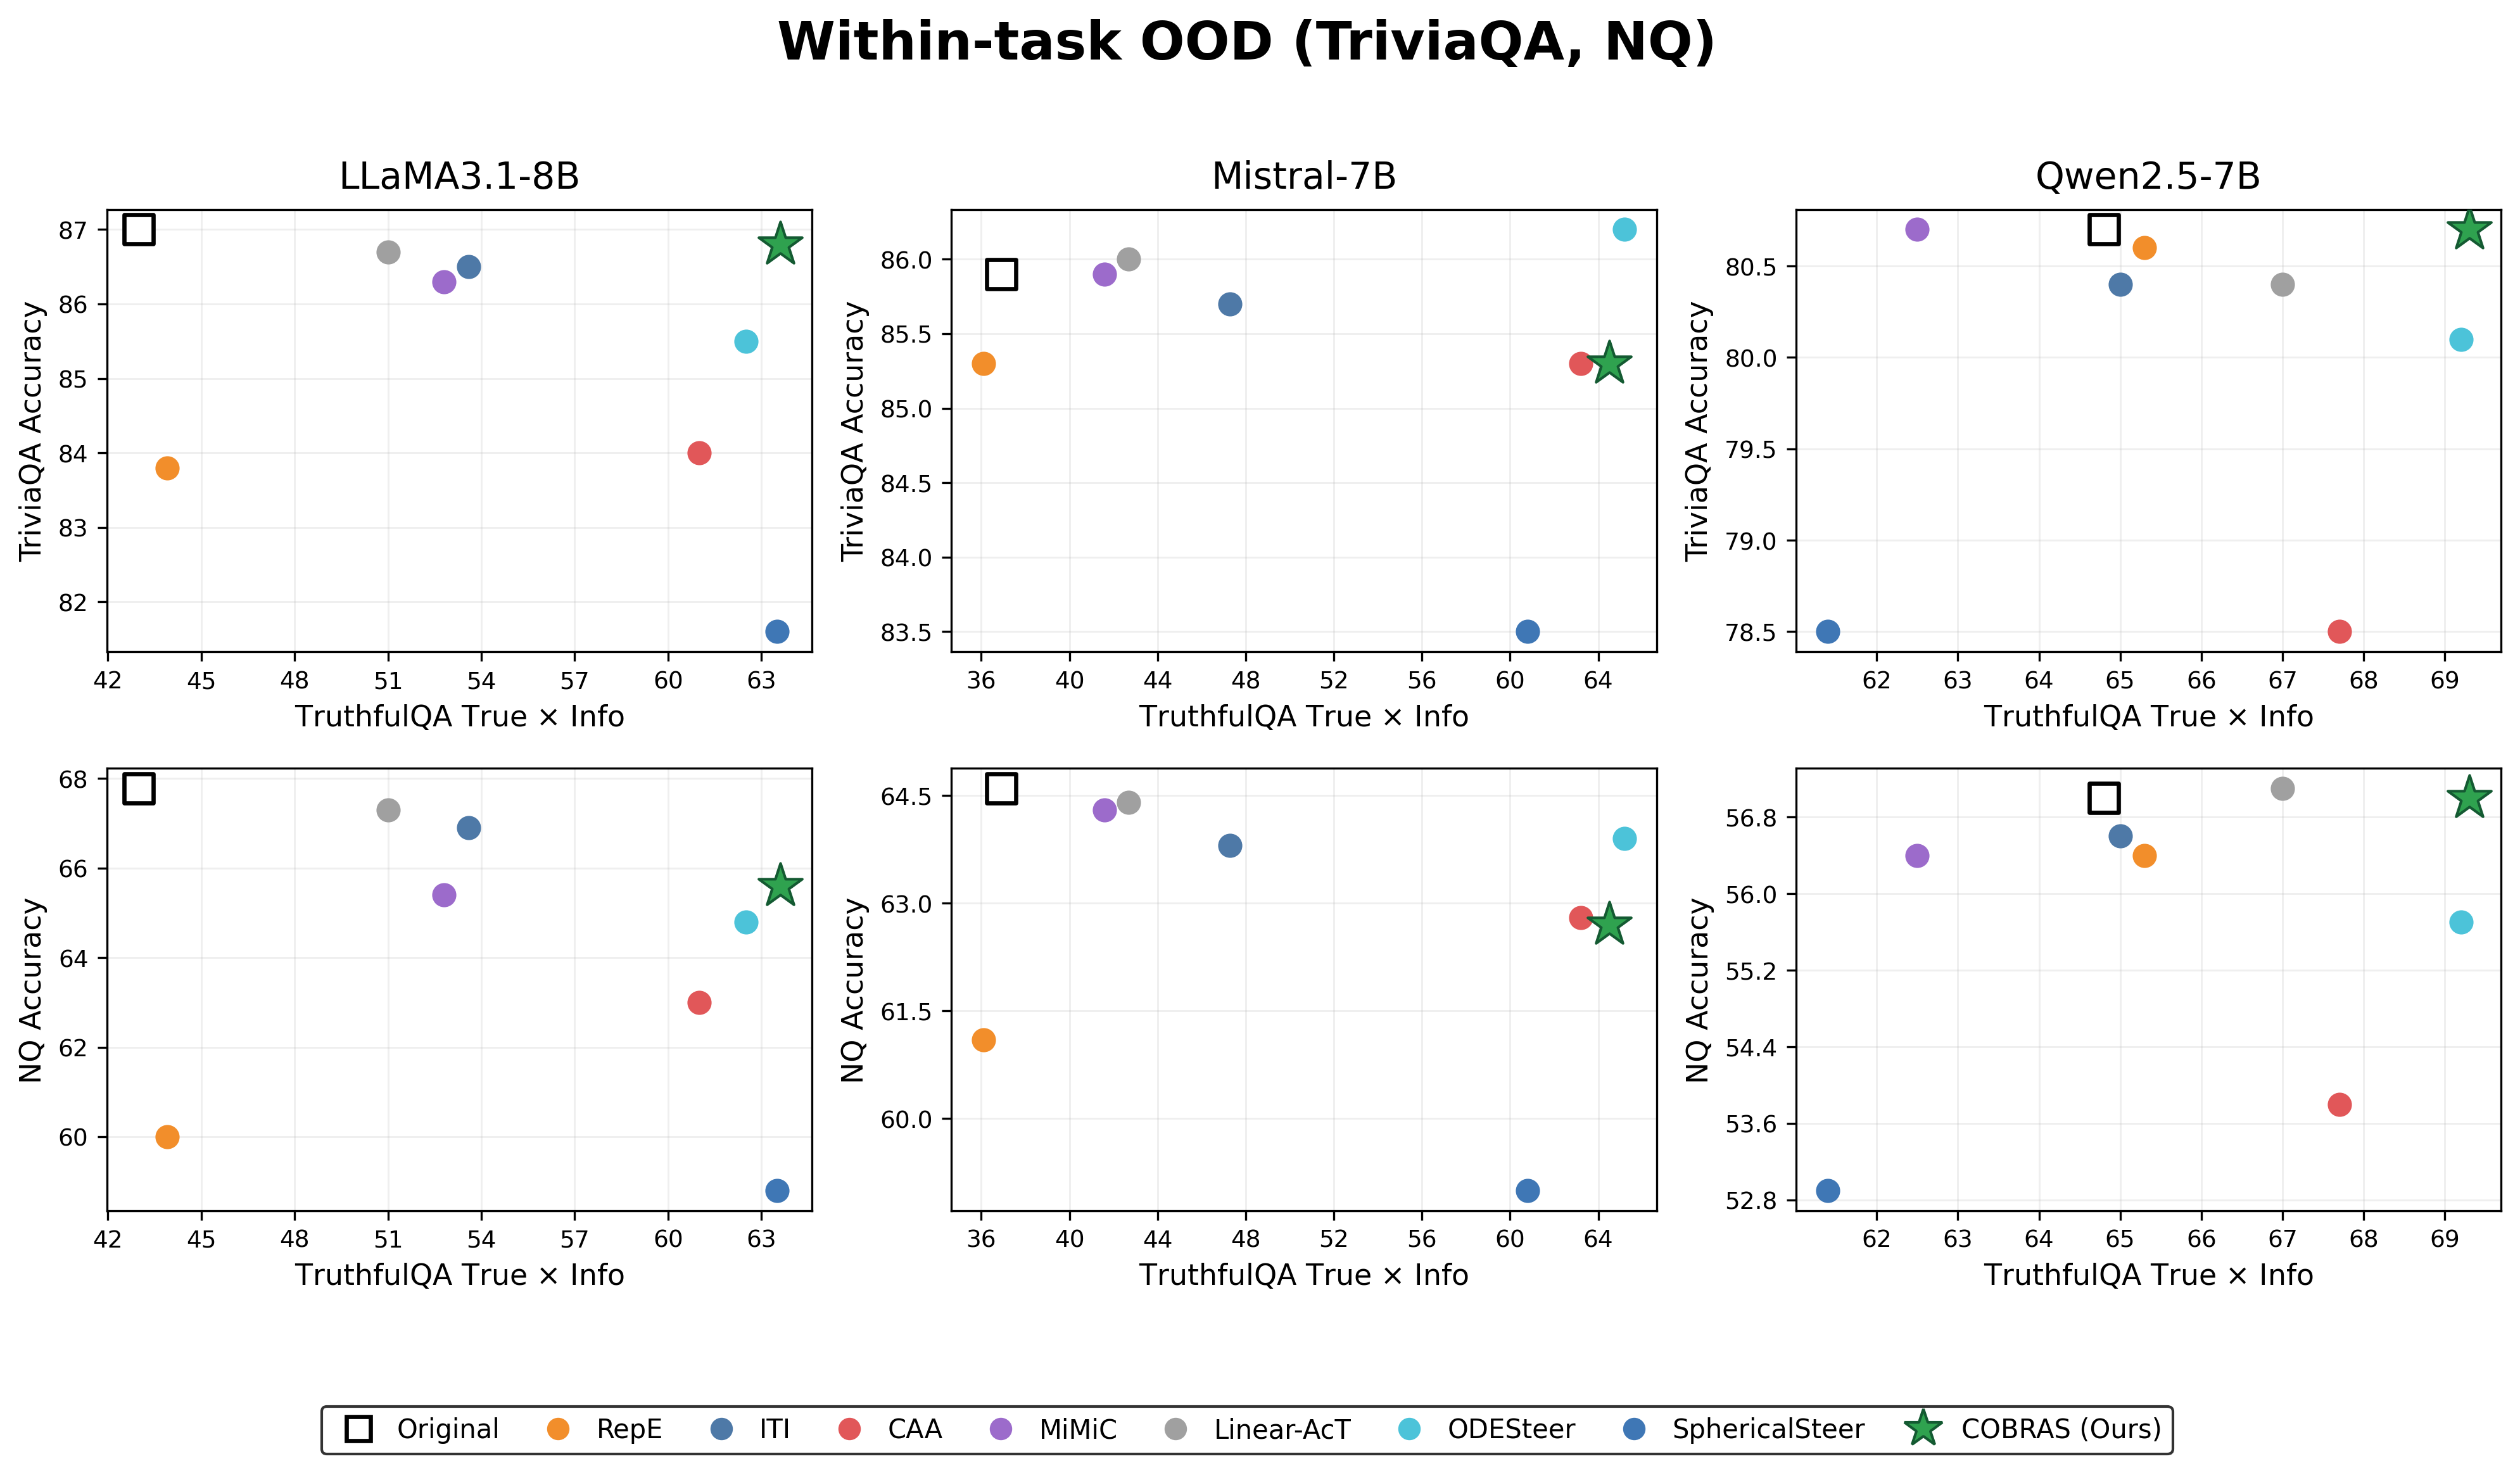
\includegraphics[width=\linewidth]{figures/within_task_ood1.png}
    \caption{Within-task OOD evaluation. Answer-ranking accuracy on TriviaQA~\citep{joshi2017triviaqa} and NQ~\citep{kwiatkowski2019natural} is plotted against TruthfulQA True$\times$Info. Falcon-7B is omitted due to its low unsteered performance.}
    \label{fig:within_task_ood}\vspace{-5mm}
\end{figure}

\noindent\textbf{RQ1: In-distribution steering performance.}~We first evaluate \Cobras in the standard in-distribution setting, where each steering method is trained and tested on the same task axis. We consider three representative alignment objectives: helpfulness on UltraFeedback, truthfulness on TruthfulQA, and detoxification on RealToxicityPrompts. Table~\ref{tab:main_results} reports results across four models.

\Cobras improves the primary metric over the unsteered model for all three tasks across models. On helpfulness, it achieves the highest mean UltraFeedback win rate for every model, improving over the original model by $+2.8$, $+7.1$, $+9.7$, and $+1.9$ absolute points on Falcon-7B, Mistral-7B, LLaMA3.1-8B, and Qwen2.5-7B, respectively. On truthfulness, it obtains the highest mean TruthfulQA True$\times$Info score across all four models, with especially large gains on Mistral-7B $(+29.5)$ and LLaMA3.1-8B $(+25.1)$. On detoxification, it reduces toxicity by approximately $41\%$--$54\%$ relative to the original models and has the lowest mean toxicity on three of four models. On Falcon-7B, CAA reduces toxicity further ($0.076$ versus $0.138$) but has substantially higher perplexity ($75.550$ versus $15.304$).
% Compared to prior steering baselines, \Cobras provides the most consistent gains across objectives. While some baselines perform well on individual tasks, they often introduce undesirable trade-offs, such as reduced informativeness on TruthfulQA or large perplexity increases on RealToxicityPrompts. In contrast, \Cobras improves the target alignment metrics while largely preserving generation quality, as reflected by competitive reward-model scores, informativeness, perplexity, and diversity. These results show that \Cobras is a strong and robust in-distribution steering method across helpfulness, truthfulness, and detoxification.

Compared to prior steering baselines, \Cobras delivers the most consistent gains across objectives. While other methods can perform well on individual tasks, they often trade off informativeness, perplexity, or diversity. In contrast, \Cobras improves target alignment metrics while largely preserving generation quality, making it a robust in-distribution steering method across helpfulness, truthfulness, and detoxification.

\noindent\textbf{RQ2: Performance under distribution shift.}~Activation steering can be brittle under distribution shift, with prior work showing that steering vectors may be unreliable in-distribution and can misgeneralize out-of-distribution ~\citep{tan2024analysing,braun2025understanding,korznikov2025rogue}. We therefore evaluate whether \Cobras improves TruthfulQA performance without degrading other capabilities by conducting experiments on both (i) within-task OOD and (ii) cross-task OOD, using the support gate in Eq.~\eqref{eq:gate} for \Cobras.


\noindent\textbf{Within-task OOD.}~In this experiment, we evaluate the performance of steering methods on two datasets, Natural Questions (NQ)~\cite{kwiatkowski2019natural} and TriviaQA~\cite{joshi2017triviaqa}, relevant to truthfulness by training only on TruthfulQA. Figure~\ref{fig:within_task_ood} plots OOD accuracy against TruthfulQA True$\times$Info; the ideal method appears in the upper-right, improving truthfulness while preserving OOD accuracy. While most methods move substantially along the TruthfulQA axis, their behavior on TriviaQA and NQ varies considerably, with some producing marked accuracy losses—most visibly on NQ. \Cobras shows a different pattern: across all three models, it attains the largest TruthfulQA improvements while keeping performance on both OOD datasets near the top of the corresponding plots. These results suggest that the gains from \Cobras are not limited to the training distribution and transfer with minimal disruption to closely related QA capabilities.

In this experiment, we evaluate the performance of steering methods on Natural Questions (NQ)~\cite{kwiatkowski2019natural} and TriviaQA~\cite{joshi2017triviaqa}, using steering learned exclusively from TruthfulQA. Figure~\ref{fig:within_task_ood} plots OOD answer-ranking accuracy against TruthfulQA True$\times$Info, where the upper-right region represents a favorable trade-off between in-distribution steering effectiveness and OOD capability retention. Several baselines achieve substantial TruthfulQA improvements but incur noticeable accuracy losses on NQ and TriviaQA, particularly SphericalSteer and CAA. In contrast, \Cobras achieves among the highest TruthfulQA scores while largely preserving OOD accuracy across all three models. On LLaMA3.1-8B and Qwen2.5-7B, \Cobras maintains performance close to the unsteered models, whereas on Mistral-7B, ODESteer provides slightly better OOD accuracy. Overall, these results indicate that \Cobras can improve in-distribution truthfulness metrics while retaining much of the models' factual question-answering capability under related distribution shifts.


\begin{figure}[t]
    \centering
    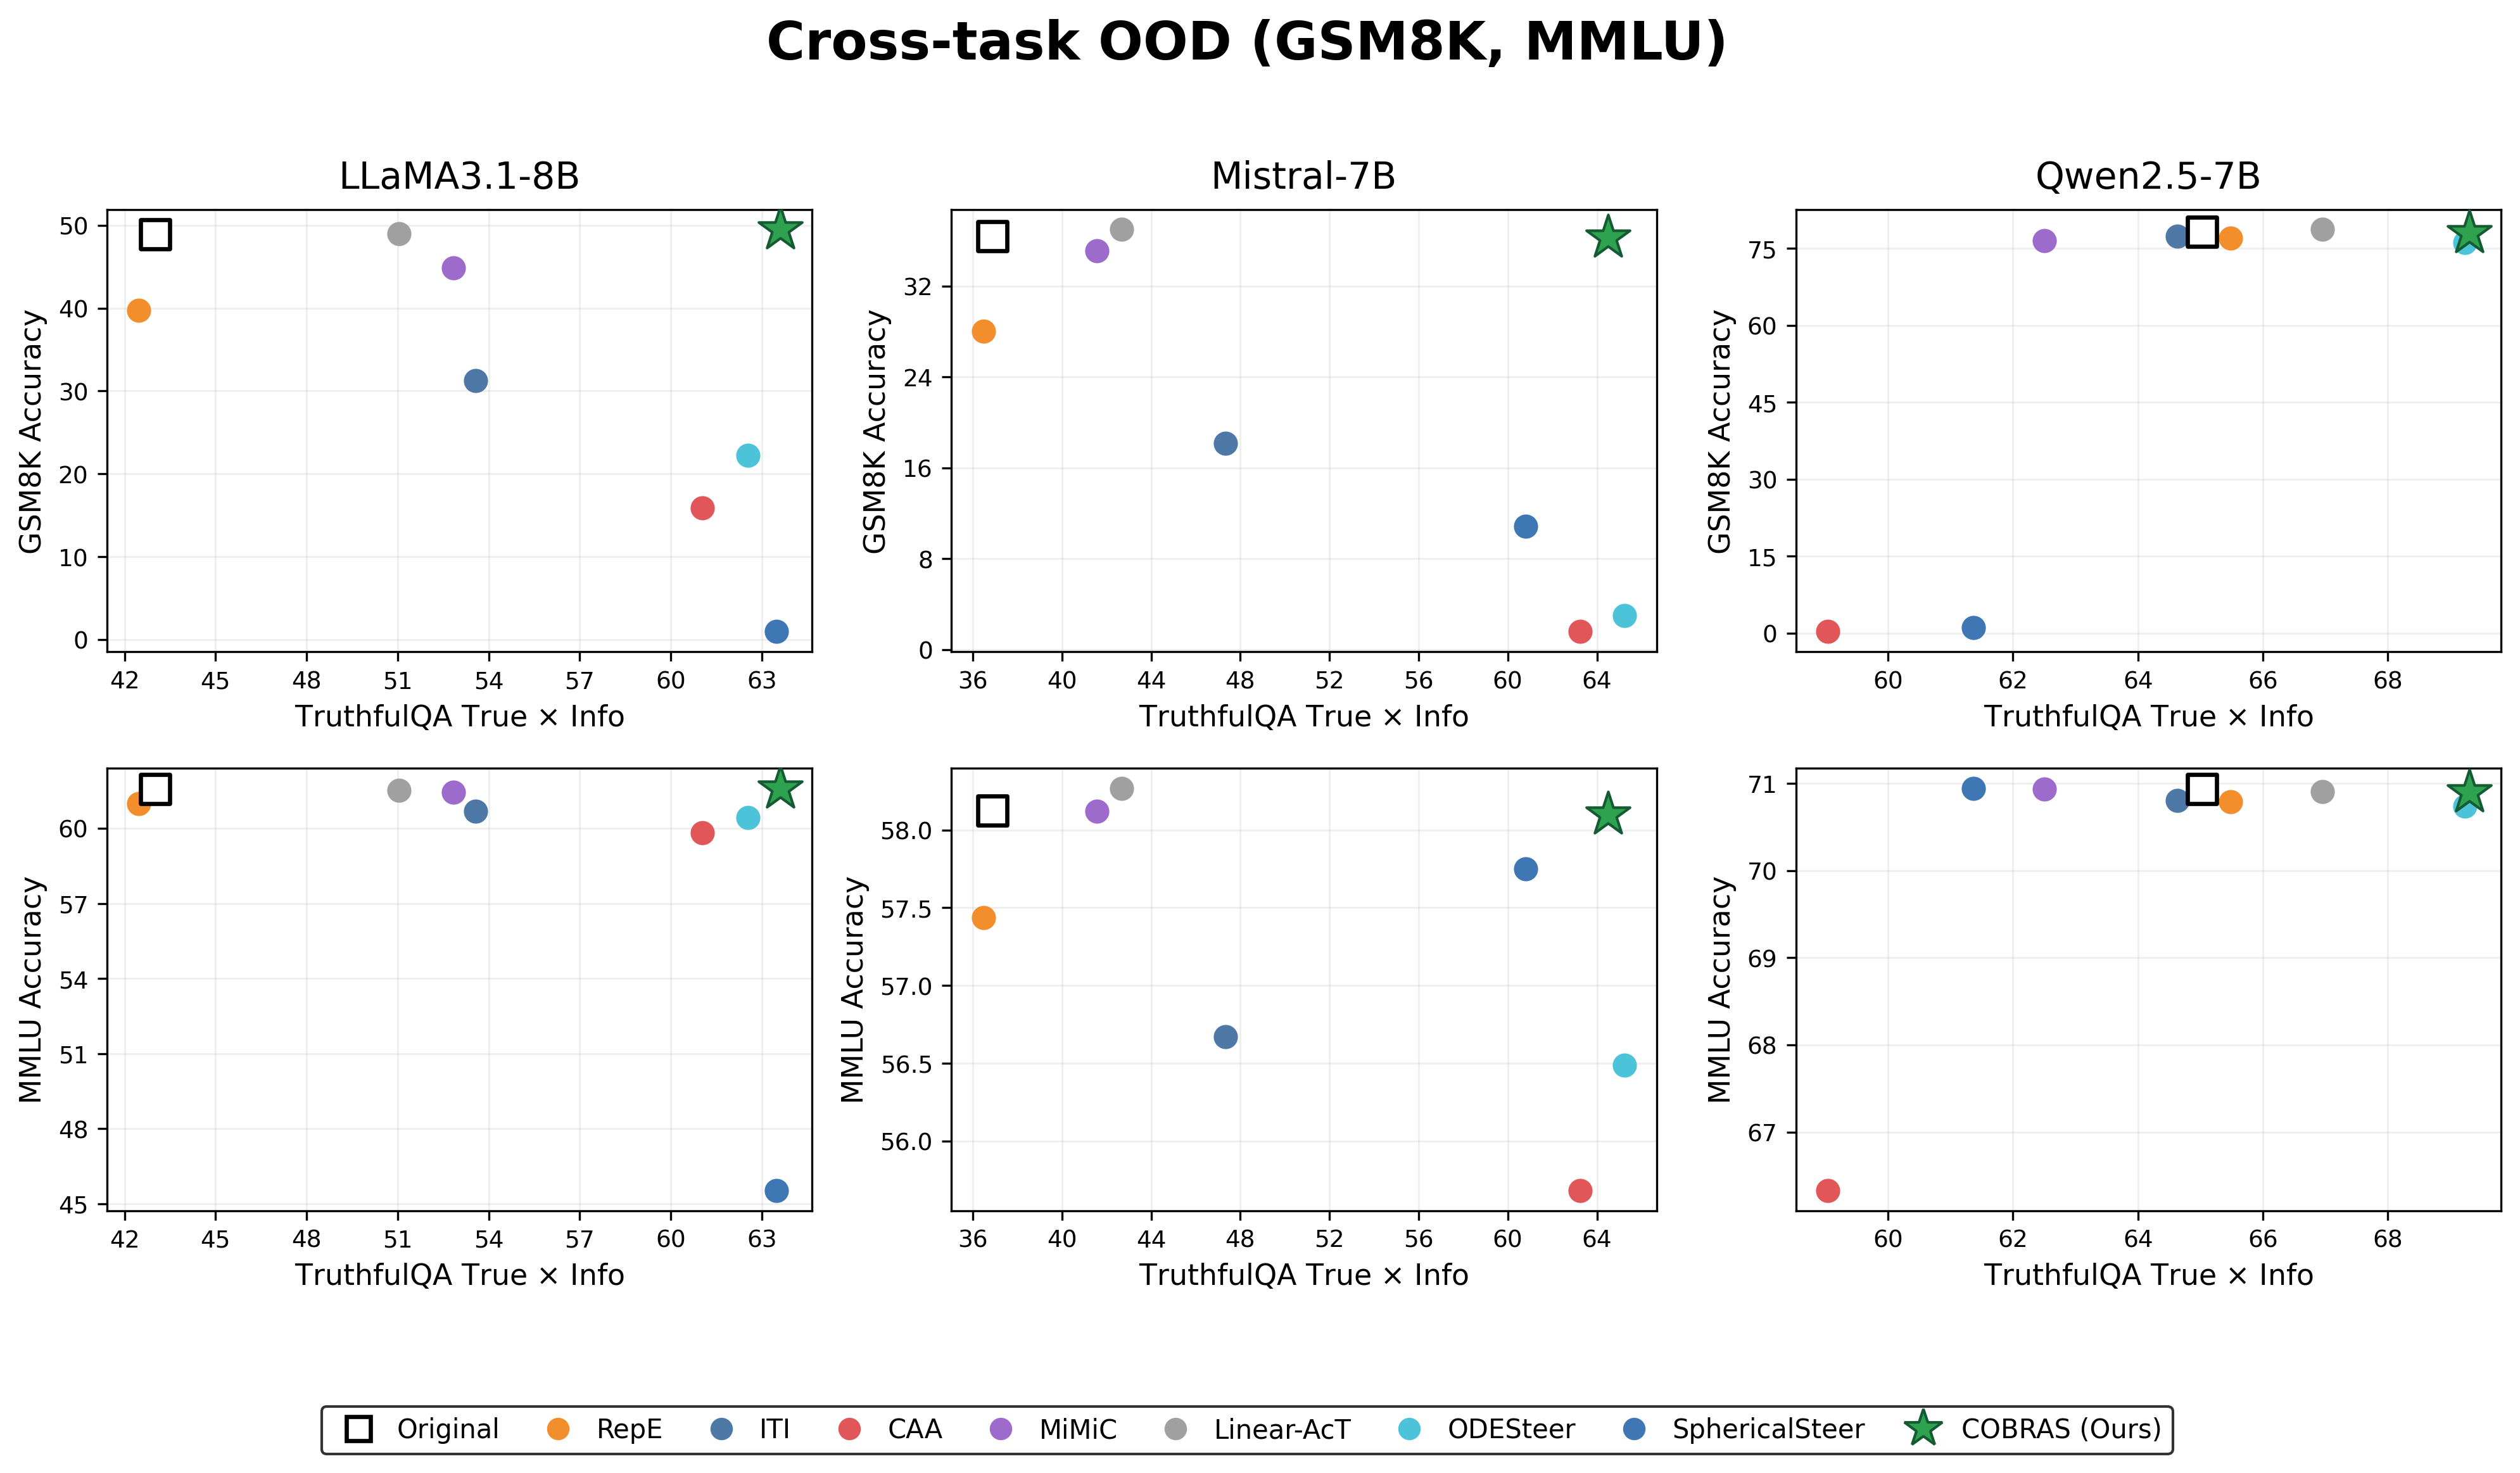
\includegraphics[width=\linewidth]{figures/cross_task_ood1.png}
    \caption{Performance of steering methods in Cross-task OOD: MMLU~\cite{hendrycks2020measuring} and GSM8K~\cite{cobbe2021gsm8k} performance. We skipped Falcon-7B because the original model's performance was low.}
    \label{fig:cross_task_ood}\vspace{-5mm}
\end{figure}

\noindent\textbf{Cross-task OOD.}~In this experiment, we train all steering methods on TruthfulQA and evaluate OOD performance on MMLU~\cite{hendrycks2020measuring} and GSM8K~\cite{cobbe2021gsm8k}. Figure~\ref{fig:cross_task_ood} plots OOD accuracy against TruthfulQA True$\times$Info; the ideal method appears in the upper-right, improving truthfulness while preserving OOD accuracy. Baselines show inconsistent trade-offs: several methods improve TruthfulQA but substantially reduce OOD performance, especially on GSM8K for LLaMA3.1-8B and Mistral-7B, and on MMLU for Mistral-7B. This suggests that some steering methods sacrifice general reasoning ability for in-distribution gains. By contrast, \Cobras consistently lies near the upper-right across all models and OOD benchmarks. It improves TruthfulQA over the original model while maintaining OOD accuracy close to, or above, the unsteered model, avoiding the severe GSM8K drops seen in several baselines. Overall, \Cobras achieves the most favorable trade-off between in-distribution steering effectiveness and OOD capability preservation.

\noindent\textbf{kNN gating across steering methods.}~We next test whether gating can also preserve OOD accuracy for other steering methods. On LLaMA3.1-8B, we compare CAA, ODESteer, SphericalSteer, and \Cobras fitted on TruthfulQA with and without a common kNN gate; for \Cobras, it replaces the support gate. Across all four methods, gating restores GSM8K and MMLU accuracy close to unsteered levels, at a cost of $1.7$--$4.0$ percentage points in TruthfulQA True$\times$Info (Table~\ref{tab:knn-external}, Appendix~\ref{apx:knn}). With this common gate, \Cobras retains the highest mean True$\times$Info ($63.6\%$ vs.\ $61.7\%$ for Spherical Steering), indicating that target-task gains still depend on the steering rule.


% \begin{figure}[!ht]
%     \centering
%     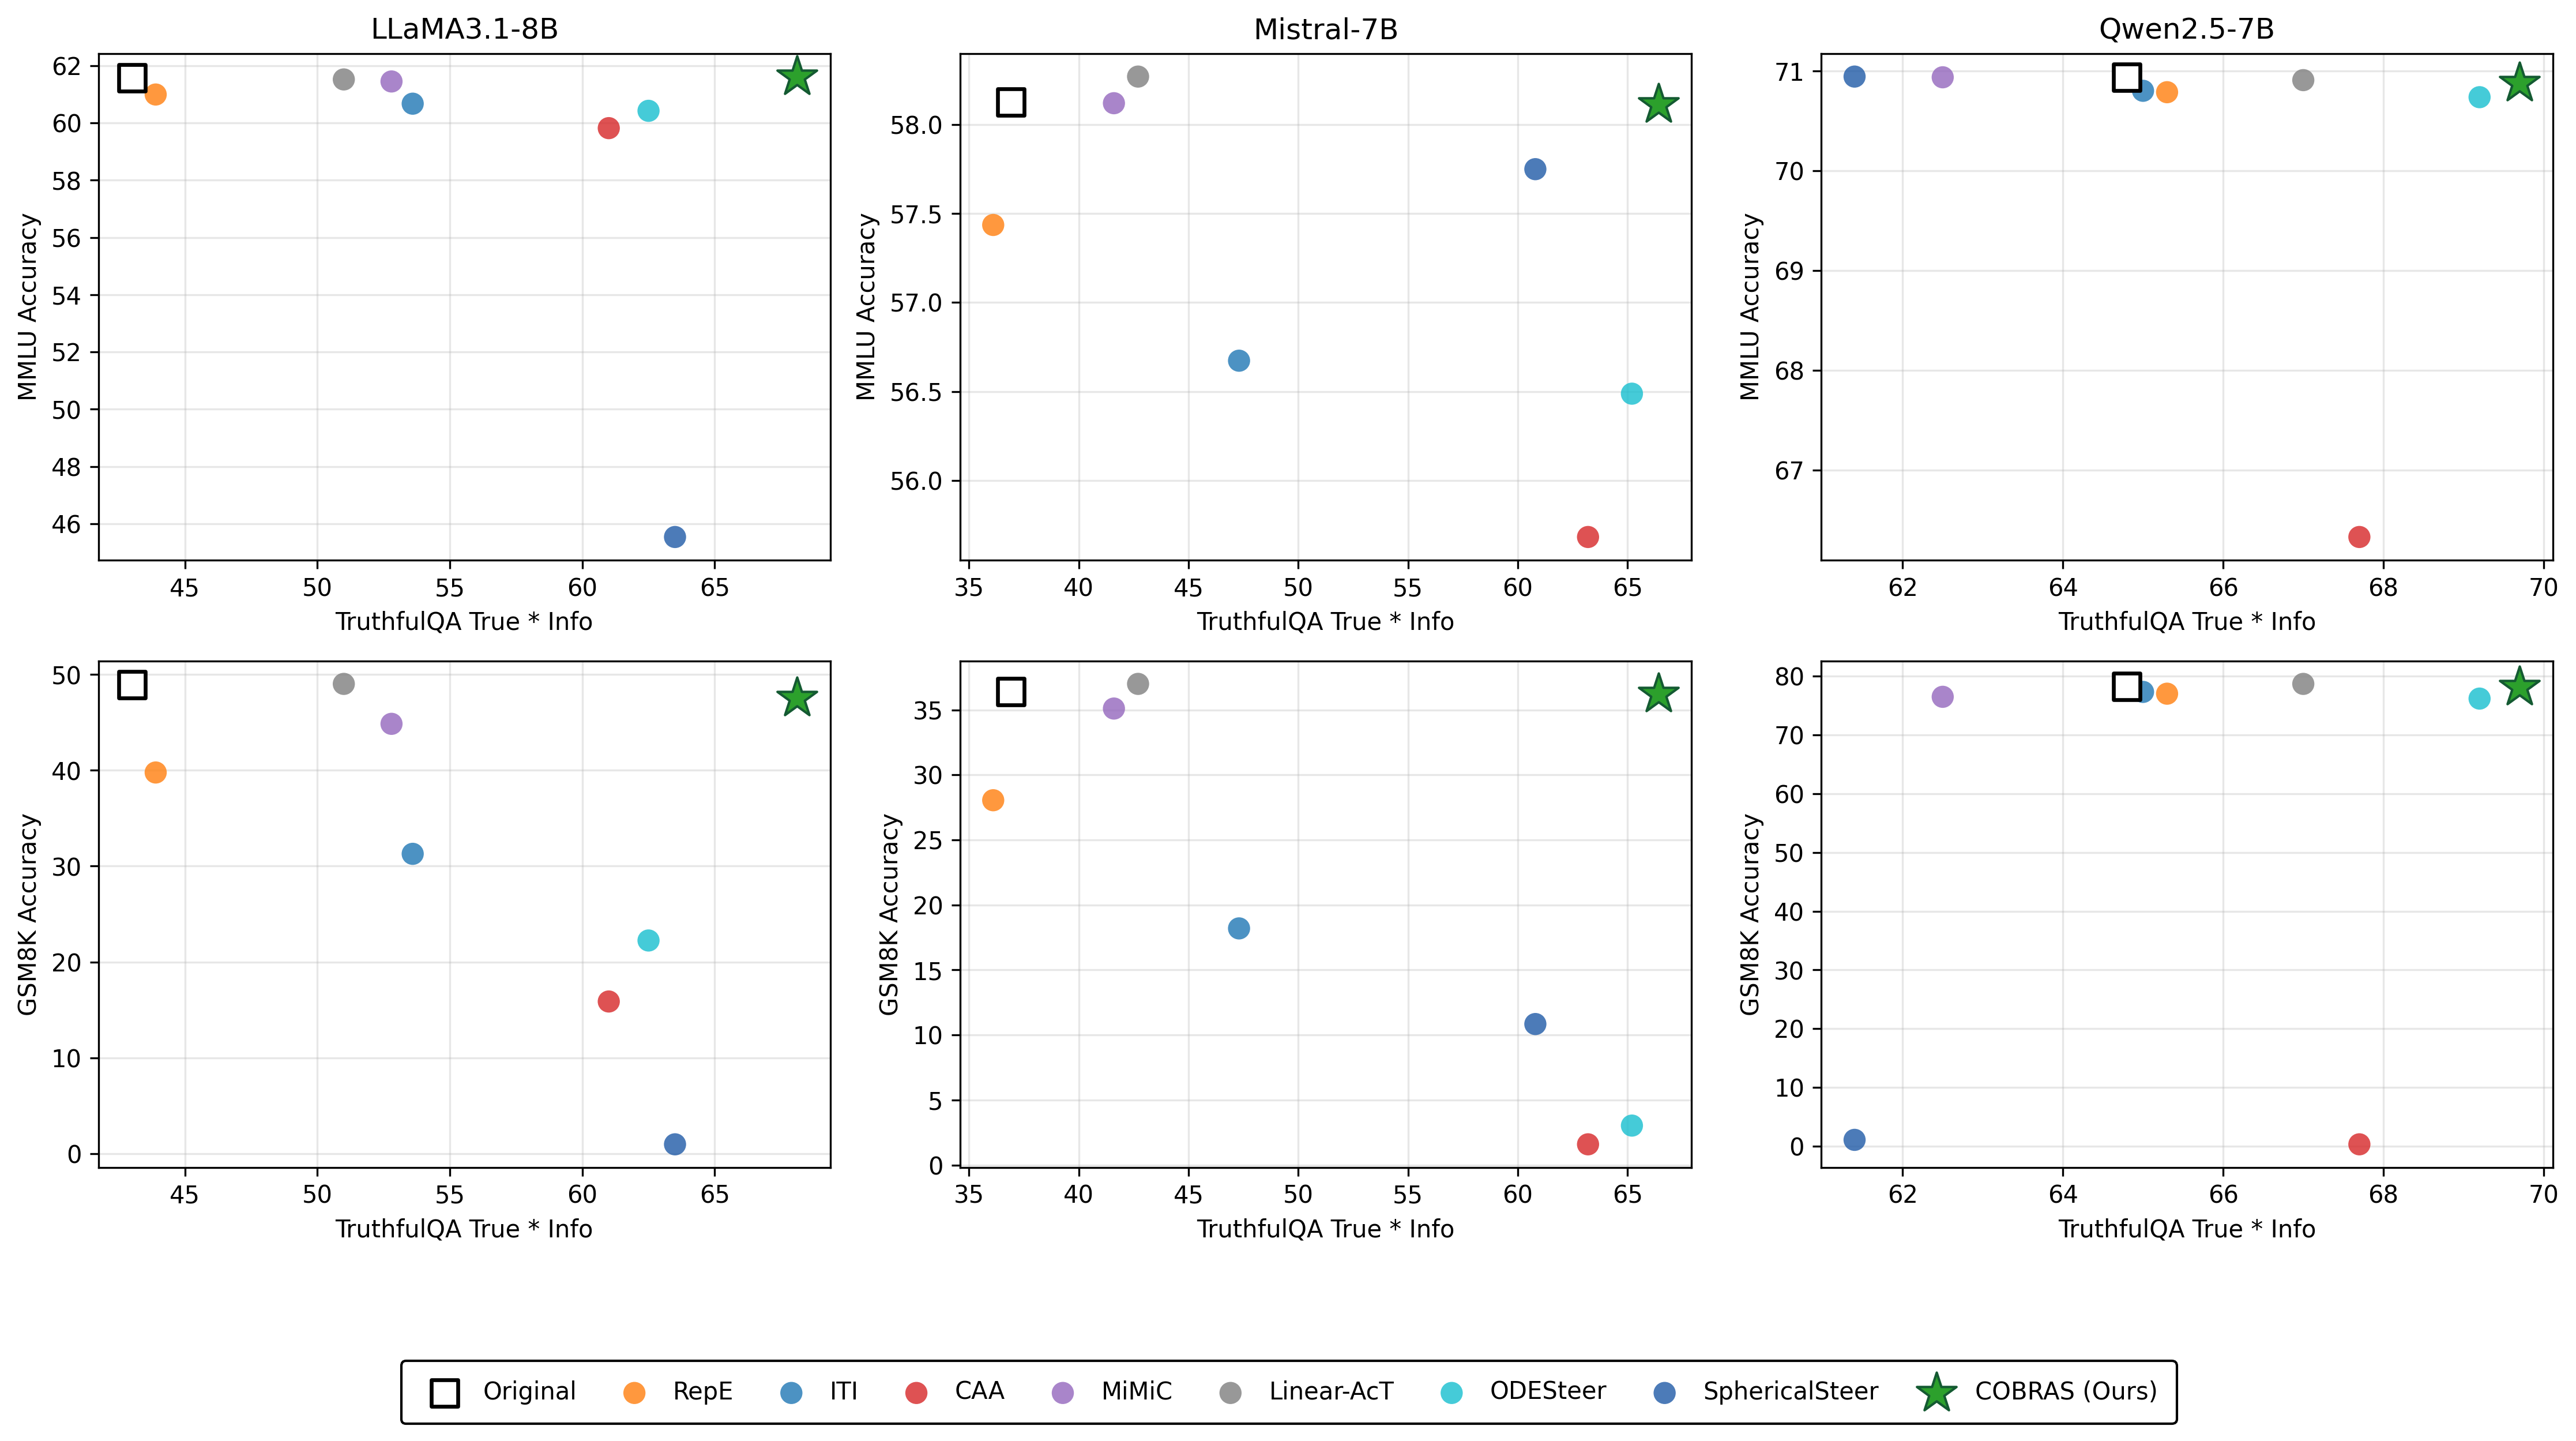
\includegraphics[width=\linewidth]{figures/tqa_vs_ood_absolute.png}
%     \caption{Performance of steering methods in OOD tasks: MMLU~\cite{hendrycks2020measuring} and GSM8K~\cite{cobbe2021gsm8k} performance. We skipped Falcon-7B because the original model's performance was low.}
%     \label{fig:ood}\vspace{-3mm}
% \end{figure}


% \paragraph{RQ3: Ablation of \Cobras Hyperparameters}
% We ablate two key hyperparameters of \Cobras, i) the abstention neighborhood size $K$, and ii) the abstention percentile. Further, ablation for Steering Strength is deferred to Appendix~\ref{appendix:cobras_vs_t}.


%\noindent\textbf{Effect of abstention parameters:} \Cobras uses an abstention rule to avoid steering inputs far from the training distribution. For each training example, we compute the distance to its $K$-th nearest neighbor and set the abstention threshold to a chosen percentile of these distances. At test time, \Cobras abstains from steering when an input's neighborhood distance exceeds this threshold. In-distribution inputs are expected to have nearby neighbors and therefore be steered, whereas OOD inputs should have larger distances and trigger abstention. Table~\ref{tab:abstain-results} evaluate this mechanism on LLaMA3.1-8B-Base and Mistral-7B-Base using TruthfulQA as the in-distribution task and GSM8K as the OOD task. Increasing the abstention percentile makes \Cobras steer more examples. This improves TruthfulQA True$\times$Info, but can reduce OOD accuracy, most notably for LLaMA3.1-8B-Base at the $99.5$th percentile. Increasing $K$ shows a similar trade-off: larger neighborhoods improve TruthfulQA, but can lower GSM8K accuracy, especially for LLaMA3.1-8B-Base. These results show that abstention helps balance effective in-distribution steering with preserving OOD capabilities.

\noindent{\textbf{RQ3: Ablations and computational cost.}}~We examine how each component of \Cobras affects its performance. On LLaMA3.1-8B, removing the support gate weakens OOD retention. Using Euclidean geometry instead of Riemannian geometry decreases performance on both in-distribution and OOD data, while removing the alignment coefficient reduces informativeness (Appendix~\ref{apx:component-ablations}). Coverage $p$ tunes the OOD trade-off (Appendix~\ref{apx:ood-gate}). Sweeps vary the integration horizon $T$, integration steps $K$, and vMF concentration $\kappa$ (Appendices~\ref{appendix:cobras_vs_t}--\ref{appendix:cobras_vs_kappa}). We also analyzed the computational overhead and potential mitigations: using $25\%$ of each contrastive dataset and $K=2$ lowers decoding overhead from $32\%$ to $7\%$ with a $1.8$-point True$\times$Info loss (Appendix~\ref{apx:computational-cost} for more details).



% Figure~\ref{fig:cobras_vs_t} shows the effect of varying the steering strength $T$ from $0.1$ to $1.0$ on TruthfulQA and UltraFeedback. On TruthfulQA, most models exhibit a clear non-monotonic trend: increasing $T$ initially improves True$\times$Info, but overly large values eventually degrade performance. LLaMA3.1-8B peaks around $T=0.6$, Mistral-7B around $T=0.7$, and Qwen2.5-7B around $T=0.4$, while Falcon-7B remains comparatively weaker and flatter before dropping sharply at high $T$. This suggests that moderate steering is sufficient for truthfulness, whereas excessive steering can overcorrect model behavior.\\
% On UltraFeedback, the effect of $T$ is more model-dependent. LLaMA3.1-8B maintains high win rate for moderate values of $T$ and peaks near $T=0.3$--$0.5$, while Falcon-7B remains relatively stable across the full range. In contrast, Mistral-7B and Qwen2.5-7B generally degrade as $T$ increases, indicating that stronger steering can harm preference-aligned generation quality. Across both datasets, these results motivate using a moderate steering strength, with the best values typically lying around $T=0.5$--$0.7$ for TruthfulQA and lower-to-moderate values for UltraFeedback.




% \begin{table}[ht]
%   \centering
%     \caption{Effect of varying the abstention percentile on LLaMA3.1-8B-Base and Mistral-7B-Base, with abstention neighborhood size fixed to $K=32$.}
%   \label{tab:abstain-percentile-results}
%     \resizebox{\linewidth}{!}{%
%       \begin{tabular}{ccccc}
%         \toprule
%         & \multicolumn{2}{c}{LLaMA3.1-8B-Base} & \multicolumn{2}{c}{Mistral-7B-Base} \\
%         \cmidrule(lr){2-3} \cmidrule(lr){4-5}
%         Abstain Percentile 
%         & TQA: T$\times$I (\%) 
%         & GSM8K: Accuracy (\%) 
%         & TQA: T$\times$I (\%) 
%         & GSM8K: Accuracy (\%) \\
%         \midrule
%         90.0  & 44.67 & 48.67 & 36.23 & 36.89 \\
%         95.0  & 54.83 & 48.90 & 37.08 & 36.31 \\
%         98.0  & 65.48 & 47.53 & 42.71 & 36.23 \\
%         99.5  & 69.15 & 11.59 & 59.48 & 35.53 \\
%         \bottomrule
%       \end{tabular}
%     }
% \end{table}

% \begin{table}[ht]
%   \centering
%   \caption{Effect of varying the abstention neighborhood size $K$ on LLaMA3.1-8B-Base and Mistral-7B-Base, with abstention percentile fixed to $98.0$.}
%   \label{tab:abstain-k-results}
%     \resizebox{\linewidth}{!}{%
%       \begin{tabular}{ccccc}
%         \toprule
%         & \multicolumn{2}{c}{LLaMA3.1-8B-Base} & \multicolumn{2}{c}{Mistral-7B-Base} \\
%         \cmidrule(lr){2-3} \cmidrule(lr){4-5}
%         Abstain $K$
%         & TQA: T$\times$I (\%) 
%         & GSM8K: Accuracy (\%) 
%         & TQA: T$\times$I (\%) 
%         & GSM8K: Accuracy (\%) \\
%         \midrule
%         32   & 65.48 & 47.53 & 42.71 & 36.23 \\
%         128  & 68.91 & 25.92 & 49.81 & 36.51 \\
%         256  & 69.40 & 15.08 & 52.50 & 36.90 \\
%         \bottomrule
%       \end{tabular}
%     }
% \end{table}


% REMOVED
% \begin{table}[ht]
%   \centering
%   \vspace{-2mm}
%   \caption{Effect of abstention parameters on LLaMA3.1-8B-Base and Mistral-7B-Base. Percentile ablations fix $K=32$, while $K$ ablations fix the abstention percentile to $98.0$.}
%   \label{tab:abstain-results}
%   \resizebox{\linewidth}{!}{%
%   % \small
%     \begin{tabular}{cccccc}
%       \toprule
%       \multirow{2}{*}{Ablation}
%       & \multirow{2}{*}{Value}
%       & \multicolumn{2}{c}{LLaMA3.1-8B-Base} 
%       & \multicolumn{2}{c}{Mistral-7B-Base} \\
%       \cmidrule(lr){3-4} \cmidrule(lr){5-6}
%       &
%       & TQA: T$\times$I (\%) ($\uparrow$)
%       & GSM8K: Acc. (\%) ($\uparrow$)
%       & TQA: T$\times$I (\%) ($\uparrow$) 
%       & GSM8K: Acc. (\%) ($\uparrow$)\\
%       \midrule

%       \multirow{4}{*}{Percentile}
%       & $90.0$  & 44.67 & 48.67 & 36.23 & 36.89 \\
%       & $95.0$  & 54.83 & 48.90 & 37.08 & 36.31 \\
%       & $98.0$  & 65.48 & 47.53 & 42.71 & 36.23 \\
%       & $99.5$  & 69.15 & 11.59 & 59.48 & 35.53 \\

%       \midrule

%       \multirow{3}{*}{$K$}
%       & $32$   & 65.48 & 47.53 & 42.71 & 36.23 \\
%       & $128$  & 68.91 & 25.92 & 49.81 & 36.51 \\
%       & $256$  & 69.40 & 15.08 & 52.50 & 36.90 \\

%       \bottomrule
%     \end{tabular}\vspace{-2mm}
%   }
% \end{table}

% \begin{table*}[!h]
% \label{tab:main_results}
% \centering
% \scriptsize
% \caption{Comparison of methods on multiple base models for helpfulness, truthfulness, and detoxification.\textcolor{red}{Arshan will update TQA , Ajay will update UF and Toxicity Eval}}
% \setlength{\tabcolsep}{3.5pt}
% \renewcommand{\arraystretch}{1.12}
% \resizebox{\textwidth}{!}{%
% \begin{tabular}{lc|ccc|ccc|ccc}
% \toprule
% \multirow{2}{*}{\textbf{Method}} & \multirow{2}{*}{\textbf{Model}} 
% & \multicolumn{3}{c|}{\textbf{Helpfulness} (\textit{UltraFeedback})}
% & \multicolumn{3}{c|}{\textbf{Truthfulness} (\textit{TruthfulQA})}
% & \multicolumn{3}{c}{\textbf{Detoxification} (\textit{Real Toxicity Prompts})} \\
% & 
% & Win (\%) $\uparrow$ & RM$_{\text{mean}}$ $\uparrow$ & RM$_{p90}$ $\uparrow$
% & T$\times$I (\%) $\uparrow$ & True (\%) $\uparrow$ & Info (\%) $\uparrow$
% & Toxic $\downarrow$ & PPL $\downarrow$ & Dist-2 $\uparrow$ \\
% \midrule

% Original & \multirow{10}{*}{\rotatebox[origin=c]{90}{LLaMA3.1-8B}}
% & 50.0 {\tiny $\pm$ 0.000} & -10.303 {\tiny $\pm$ 0.145} & -0.744 {\tiny $\pm$ 0.435} 
% & 43.0 {\tiny $\pm$ 1.496} & 45.1 {\tiny $\pm$ 1.309} & 97.6 {\tiny $\pm$ 0.628}
% & 0.218 {\tiny $\pm$ 0.002} & 18.562 {\tiny $\pm$ 0.107} & 0.992 {\tiny $\pm$ 0.001}  \\\midrule


% RepE &
% & 47.1 {\tiny $\pm$ 1.050} & -10.763 {\tiny $\pm$ 0.295} & -1.356 {\tiny $\pm$ 0.378} 
% & 43.9 {\tiny $\pm$ 1.041} & 46.2 {\tiny $\pm$ 0.989} & 97.4 {\tiny $\pm$ 0.187}
% & 0.195 {\tiny $\pm$ 0.003} & 19.101 {\tiny $\pm$ 0.496} & 0.991 {\tiny $\pm$ 0.001} \\

% ITI &
% & 51.5 {\tiny $\pm$ 2.026} & -10.138 {\tiny $\pm$ 0.232} & -0.739 {\tiny $\pm$ 0.611} 
% & 53.6 {\tiny $\pm$ 1.055} & 57.3 {\tiny $\pm$ 0.902} & 95.8 {\tiny $\pm$ 0.374}
% & 0.190 {\tiny $\pm$ 0.011} & 18.698 {\tiny $\pm$ 0.377} & 0.990 {\tiny $\pm$ 0.002} \\

% CAA &
% & 50.9 {\tiny $\pm$ 0.874} & -9.966 {\tiny $\pm$ 0.132} & -0.628 {\tiny $\pm$ 0.380} 
% & 61.0 {\tiny $\pm$ 2.020} & 68.1 {\tiny $\pm$ 2.221} & 92.6 {\tiny $\pm$ 0.495}
% & 0.152 {\tiny $\pm$ 0.005} & 19.647 {\tiny $\pm$ 0.349} & 0.992 {\tiny $\pm$ 0.001} \\

% MiMiC &
% & 54.9 {\tiny $\pm$ 1.905} & -9.713 {\tiny $\pm$ 0.175} & -0.549 {\tiny $\pm$ 0.112} 
% & 52.8 {\tiny $\pm$ 1.041} & 60.1 {\tiny $\pm$ 0.430} & 92.0 {\tiny $\pm$ 0.612}
% & 0.198 {\tiny $\pm$ 0.010} & 18.667 {\tiny $\pm$ 0.311} & 0.991 {\tiny $\pm$ 0.001} \\

% Linear-AcT &
% & 52.5 {\tiny $\pm$ 2.203} & -9.944 {\tiny $\pm$ 0.469} & -0.411 {\tiny $\pm$ 0.654}
% & 51.0 {\tiny $\pm$ 1.484} & 53.1 {\tiny $\pm$ 1.683} & 97.8 {\tiny $\pm$ 0.187}
% & 0.199 {\tiny $\pm$ 0.014} & 18.521 {\tiny $\pm$ 0.333} & 0.991 {\tiny $\pm$ 0.001} \\

% ODESteer &
% & 56.3 {\tiny $\pm$ 0.896} & -8.280 {\tiny $\pm$ 0.316} & 1.206 {\tiny $\pm$ 0.441} & 62.5 {\tiny $\pm$ 2.570} & 67.3 {\tiny $\pm$ 2.544} & 95.1 {\tiny $\pm$ 0.441}
% & 0.124 {\tiny $\pm$ 0.002} & 19.831 {\tiny $\pm$ 0.224} & 0.993 {\tiny $\pm$ 0.000}  \\

% SphericalSteer &
% & 52.3 {\tiny $\pm$ 1.790} & -9.434 {\tiny $\pm$ 0.304} & -0.633 {\tiny $\pm$ 0.837} & 63.5 {\tiny $\pm$ 0.902} & 86.9 {\tiny $\pm$ 2.389} & 76.0 {\tiny $\pm$ 1.504} 
% & 0.123 {\tiny $\pm$ 0.010} & 23.039 {\tiny $\pm$ 0.274} & 0.993 {\tiny $\pm$ 0.000} \\

% \midrule

% \textbf{COBRAS (Ours)} &
% & \textbf{59.7} {\tiny $\pm$ 1.610}  & -8.109 {\tiny $\pm$ 0.283}  &  0.800 {\tiny $\pm$ 0.120}
% & \textbf{68.1} {\tiny $\pm$ 1.343} & 82.8 {\tiny $\pm$ 0.308} & 84.9 {\tiny $\pm$ 1.168}
% & 0.107 {\tiny $\pm$ 0.004} & 20.083 {\tiny $\pm$ 0.184} & 0.992 {\tiny $\pm$ 0.000} \\

% \midrule
% \midrule
% Original & \multirow{10}{*}{\rotatebox[origin=c]{90}{Falcon-7B}}
% & 50.0 {\tiny $\pm$ 0.000} & -12.642 {\tiny $\pm$ 0.162} & -2.705 {\tiny $\pm$ 0.171} 
% & 29.1 {\tiny $\pm$ 0.919} & 32.1 {\tiny $\pm$ 0.951} & 96.5 {\tiny $\pm$ 0.283} 
% & 0.255 {\tiny $\pm$ 0.004} & 15.358 {\tiny $\pm$ 0.449} & 0.946 {\tiny $\pm$ 0.003} \\\midrule



% RepE &
% & 50.2 {\tiny $\pm$ 0.981} & -12.711 {\tiny $\pm$ 0.270} & -2.680 {\tiny $\pm$ 0.099} 
% & 28.7 {\tiny $\pm$ 1.069} & 31.7 {\tiny $\pm$ 0.982} & 96.6 {\tiny $\pm$ 0.308} 
% & 0.232 {\tiny $\pm$ 0.010} & 15.371 {\tiny $\pm$ 0.178} & 0.941 {\tiny $\pm$ 0.003}  \\

% ITI &
% & 49.0 {\tiny $\pm$ 1.358} & -12.789 {\tiny $\pm$ 0.221} & -2.866 {\tiny $\pm$ 0.134} 
% & 32.8 {\tiny $\pm$ 0.616} & 36.8 {\tiny $\pm$ 0.738} & 95.5 {\tiny $\pm$ 0.393}
% & 0.239 {\tiny $\pm$ 0.004} & 15.707 {\tiny $\pm$ 0.346} & 0.941 {\tiny $\pm$ 0.005} \\

% CAA &
% & 49.9 {\tiny $\pm$ 2.346} & -12.540 {\tiny $\pm$ 0.226} & -2.260 {\tiny $\pm$ 0.410} 
% & 37.9 {\tiny $\pm$ 1.495} & 42.0 {\tiny $\pm$ 1.905} & 95.4 {\tiny $\pm$ 0.494}
% & 0.076 {\tiny $\pm$ 0.007} & 75.550 {\tiny $\pm$ 9.063} & 0.852 {\tiny $\pm$ 0.002} \\

% MiMiC &
% & 50.7 {\tiny $\pm$ 1.350} & -12.751 {\tiny $\pm$ 0.136} & -2.678 {\tiny $\pm$ 0.213} 
% & 32.9 {\tiny $\pm$ 0.764} & 43.3 {\tiny $\pm$ 0.374} & 88.3 {\tiny $\pm$ 0.927} 
% & 0.240 {\tiny $\pm$ 0.009} & 15.026 {\tiny $\pm$ 0.258} & 0.941 {\tiny $\pm$ 0.004}  \\

% Linear-AcT &
% & 50.8 {\tiny $\pm$ 1.300} & -12.412 {\tiny $\pm$ 0.205} & -2.534 {\tiny $\pm$ 0.309} 
% & 40.0 {\tiny $\pm$ 0.561} & 44.3 {\tiny $\pm$ 0.534} & 95.0 {\tiny $\pm$ 0.212}
% & 0.240 {\tiny $\pm$ 0.003} & 16.113 {\tiny $\pm$ 0.206} & 0.947 {\tiny $\pm$ 0.002} \\


% ODESteer &
% & 49.7 {\tiny $\pm$ 1.210} & -12.446 {\tiny $\pm$ 0.050} & -2.806 {\tiny $\pm$ 0.207} 
% & 32.1 {\tiny $\pm$ 0.674} & 35.4 {\tiny $\pm$ 0.534} & 96.2 {\tiny $\pm$ 0.441} 
% & 0.188 {\tiny $\pm$ 0.006} & 15.709 {\tiny $\pm$ 0.405} & 0.940 {\tiny $\pm$ 0.002} \\

% SphericalSteer &
% & 49.5 {\tiny $\pm$ 2.255} & -12.495 {\tiny $\pm$ 0.120} & -3.108 {\tiny $\pm$ 0.244} 
% & 37.7 {\tiny $\pm$ 1.354} & 62.9 {\tiny $\pm$ 1.469} & 71.6 {\tiny $\pm$ 1.534} 
% & 0.147 {\tiny $\pm$ 0.011} & 21.542 {\tiny $\pm$ 1.543} & 0.924 {\tiny $\pm$ 0.008} \\

% \midrule
% \textbf{COBRAS (Ours)} &
% & \textbf{52.8} {\tiny $\pm$ 2.628}  &  -12.24 {\tiny $\pm$ 0.336}  & -2.60 {\tiny $\pm$ 0.121}  
% & \textbf{40.3} {\tiny $\pm$ 1.390} & 45.5 {\tiny $\pm$ 2.124} & 93.4 {\tiny $\pm$ 1.379}
% & 0.138 {\tiny $\pm$ 0.012} & 15.304 {\tiny $\pm$ 0.591} & 0.942 {\tiny $\pm$ 0.005} \\

% \midrule
% \midrule
% Original & \multirow{10}{*}{\rotatebox[origin=c]{90}{Mistral-7B}}
% & 50.0 {\tiny $\pm$ 0.000} & -11.063 {\tiny $\pm$ 0.377} & -0.469 {\tiny $\pm$ 0.752} 
% & 36.9 {\tiny $\pm$ 0.616} & 41.7 {\tiny $\pm$ 0.764} & 94.8 {\tiny $\pm$ 0.463} 
% & 0.207 {\tiny $\pm$ 0.008} & 18.542 {\tiny $\pm$ 0.498} & 0.990 {\tiny $\pm$ 0.001} \\\midrule


% RepE &
% & 45.3 {\tiny $\pm$ 2.237} & -11.981 {\tiny $\pm$ 0.377} & -1.622 {\tiny $\pm$ 0.423} 
% & 36.1 {\tiny $\pm$ 1.055} & 42.0 {\tiny $\pm$ 0.674} & 93.9 {\tiny $\pm$ 0.490} 
% & 0.218 {\tiny $\pm$ 0.004} & 76.065 {\tiny $\pm$ 1.734} & 0.969 {\tiny $\pm$ 0.001}  \\

% ITI &
% & 48.8 {\tiny $\pm$ 0.611} & -11.116 {\tiny $\pm$ 0.310} & -1.229 {\tiny $\pm$ 0.311} 
% & 47.3 {\tiny $\pm$ 1.952} & 54.2 {\tiny $\pm$ 1.616} & 92.6 {\tiny $\pm$ 1.041}
% & 0.181 {\tiny $\pm$ 0.013} & 18.956 {\tiny $\pm$ 0.170} & 0.989 {\tiny $\pm$ 0.000} \\

% CAA &
% & 53.7 {\tiny $\pm$ 4.636} & -10.424 {\tiny $\pm$ 0.144} & -0.601 {\tiny $\pm$ 0.439} 
% & 63.2 {\tiny $\pm$ 0.989} & 74.7 {\tiny $\pm$ 0.212} & 88.2 {\tiny $\pm$ 1.278}
% & 0.167 {\tiny $\pm$ 0.011} & 18.912 {\tiny $\pm$ 0.281} & 0.991 {\tiny $\pm$ 0.001}  \\

% MiMiC &
% & 48.5 {\tiny $\pm$ 2.751} & -11.511 {\tiny $\pm$ 0.324} & -0.676 {\tiny $\pm$ 0.535} 
% & 41.6 {\tiny $\pm$ 1.019} & 50.2 {\tiny $\pm$ 2.124} & 91.2 {\tiny $\pm$ 1.176}
% & 0.192 {\tiny $\pm$ 0.010} & 18.922 {\tiny $\pm$ 0.781} & 0.989 {\tiny $\pm$ 0.001}  \\


% Linear-AcT &
% & 53.0 {\tiny $\pm$ 4.996} & -10.448 {\tiny $\pm$ 0.191} & -0.139 {\tiny $\pm$ 0.544} 
% & 42.7 {\tiny $\pm$ 0.796} & 48.4 {\tiny $\pm$ 0.738} & 94.0 {\tiny $\pm$ 0.141} 
% & 0.189 {\tiny $\pm$ 0.009} & 18.784 {\tiny $\pm$ 0.320} & 0.990 {\tiny $\pm$ 0.001}  \\

% ODESteer &
% & 54.8 {\tiny $\pm$ 3.946} & -10.951 {\tiny $\pm$ 0.275} & -0.622 {\tiny $\pm$ 0.041}
% & 65.2 {\tiny $\pm$ 1.619} & 73.9 {\tiny $\pm$ 1.443} & 91.1 {\tiny $\pm$ 0.141}
% & 0.101 {\tiny $\pm$ 0.008} & 21.081 {\tiny $\pm$ 0.156} & 0.993 {\tiny $\pm$ 0.001} \\

% SphericalSteer &
% & 50.3 {\tiny $\pm$ 2.948} & -11.005 {\tiny $\pm$ 0.126} & -1.958 {\tiny $\pm$ 0.337} 
% & 60.8 {\tiny $\pm$ 1.630} & 76.6 {\tiny $\pm$ 1.324} & 83.7 {\tiny $\pm$ 0.510} 
% & 0.099 {\tiny $\pm$ 0.005} & 21.295 {\tiny $\pm$ 0.122} & 0.990 {\tiny $\pm$ 0.001} \\

% \midrule
% \textbf{COBRAS (Ours)} &
% & \textbf{57.1} {\tiny $\pm$ 3.253} & -10.261 {\tiny $\pm$ 0.163} & -0.157 {\tiny $\pm$ 0.621} 
% &  \textbf{66.4} {\tiny $\pm$ 1.901} & 85.2 {\tiny $\pm$ 0.972} & 80.3 {\tiny $\pm$ 0.982}
% & 0.096 {\tiny $\pm$ 0.006} & 20.631 {\tiny $\pm$ 0.330} & 0.992 {\tiny $\pm$ 0.001}  \\

% \midrule
% \midrule
% Original & \multirow{10}{*}{\rotatebox[origin=c]{90}{Qwen2.5-7B}}
% & 50.0 {\tiny $\pm$ 0.000} & -6.006 {\tiny $\pm$ 0.208} & 4.384 {\tiny $\pm$ 0.378} 
% & 64.8 {\tiny $\pm$ 0.707} & 78.3 {\tiny $\pm$ 0.578} & 86.4 {\tiny $\pm$ 0.764} 
% & 0.194 {\tiny $\pm$ 0.001} & 22.166 {\tiny $\pm$ 0.369} & 0.989 {\tiny $\pm$ 0.001}  \\\midrule


% RepE &
% & 48.8 {\tiny $\pm$ 0.300} & -6.011 {\tiny $\pm$ 0.202} & 4.504 {\tiny $\pm$ 0.271} 
% & 65.3 {\tiny $\pm$ 1.429} & 78.7 {\tiny $\pm$ 0.927} & 86.5 {\tiny $\pm$ 1.111} 
% & 0.196 {\tiny $\pm$ 0.002} & 22.620 {\tiny $\pm$ 0.681} & 0.990 {\tiny $\pm$ 0.000} \\

% ITI &
% & 49.9 {\tiny $\pm$ 1.054} & -6.034 {\tiny $\pm$ 0.373} & 4.349 {\tiny $\pm$ 0.408} 
% & 65.0 {\tiny $\pm$ 0.374} & 78.7 {\tiny $\pm$ 0.956} & 86.0 {\tiny $\pm$ 0.857} 
% & 0.184 {\tiny $\pm$ 0.005} & 22.617 {\tiny $\pm$ 0.895} & 0.990 {\tiny $\pm$ 0.001} \\

% CAA &
% & 50.0 {\tiny $\pm$ 1.587} & -5.957 {\tiny $\pm$ 0.072} & 4.659 {\tiny $\pm$ 0.312} 
% & 67.7 {\tiny $\pm$ 2.093} & 81.2 {\tiny $\pm$ 1.111} & 86.4 {\tiny $\pm$ 1.534} 
% & 0.114 {\tiny $\pm$ 0.005} & 28.218 {\tiny $\pm$ 1.014} & 0.982 {\tiny $\pm$ 0.002}  \\

% MiMiC &
% & 50.2 {\tiny $\pm$ 1.023 } & -5.980 {\tiny $\pm$ 0.133} & 4.753 {\tiny $\pm$ 0.312}  
% & 62.5 {\tiny $\pm$ 1.097} & 82.9 {\tiny $\pm$ 0.283} & 79.0 {\tiny $\pm$ 1.026} 
% & 0.176 {\tiny $\pm$ 0.005} & 21.233 {\tiny $\pm$ 0.363} & 0.989 {\tiny $\pm$ 0.002}  \\

% Linear-AcT &
% & 50.4 {\tiny $\pm$ 1.747} & -6.017 {\tiny $\pm$ 0.111} & 4.788 {\tiny $\pm$ 0.499} 
% & 67.0 {\tiny $\pm$ 1.168} & 79.8 {\tiny $\pm$ 1.205} & 87.0 {\tiny $\pm$ 1.046} 
% & 0.181 {\tiny $\pm$ 0.004} & 22.643 {\tiny $\pm$ 0.876} & 0.990 {\tiny $\pm$ 0.001} \\

% ODESteer &
% & 50.7 {\tiny $\pm$ 1.222} & -5.995 {\tiny $\pm$ 0.095} & 4.738 {\tiny $\pm$ 0.175} 
% & 69.2 {\tiny $\pm$ 1.434} & 82.2 {\tiny $\pm$ 1.460} & 86.7 {\tiny $\pm$ 2.145}
% & 0.170 {\tiny $\pm$ 0.004} & 22.310 {\tiny $\pm$ 0.565} & 0.990 {\tiny $\pm$ 0.002}  \\

% SphericalSteer &
% & 43.6 {\tiny $\pm$ 1.644} & -7.203 {\tiny $\pm$ 0.208} & 4.309 {\tiny $\pm$ 0.192} 
% & 61.4 {\tiny $\pm$ 2.086} & 82.9 {\tiny $\pm$ 1.874} & 77.6 {\tiny $\pm$ 1.067} 
% & 0.129 {\tiny $\pm$ 0.007} & 68.485 {\tiny $\pm$ 2.191} & 0.942 {\tiny $\pm$ 0.008} \\

% \midrule
% \textbf{COBRAS (Ours)} &
% & \textbf{51.9} {\tiny $\pm$ 1.616} &   -5.755 { \tiny$\pm$ 0.419} &    5.162 {\tiny $\pm$ 0.746}
% &  \textbf{69.7} {\tiny $\pm$ 0.495} & 83.3 {\tiny $\pm$ 0.430} & 86.8 {\tiny $\pm$ 0.141}
% & 0.119 {\tiny $\pm$ 0.006} & 23.786 {\tiny $\pm$ 0.625} & 0.985 {\tiny $\pm$ 0.003} \\

% \bottomrule
% \end{tabular}%
% }
% \label{tab:main_comparison}
% \end{table*}







% \begin{table*}[!h]
% \label{tab:main_results}
% \centering
% \scriptsize
% \caption{Comparison of methods on multiple base models for helpfulness, truthfulness, and detoxification.\textcolor{red}{Arshan will update TQA , Ajay will update UF and Toxicity Eval}}
% \setlength{\tabcolsep}{3.5pt}
% \renewcommand{\arraystretch}{1.12}
% \resizebox{\textwidth}{!}{%
% \begin{tabular}{lc|ccc|ccc|ccc}
% \toprule
% \multirow{2}{*}{\textbf{Method}} & \multirow{2}{*}{\textbf{Model}}  & \multicolumn{3}{c|}{\textbf{Helpfulness} (\textit{UltraFeedback})} & \multicolumn{3}{c|}{\textbf{Truthfulness} (\textit{TruthfulQA})} & \multicolumn{3}{c}{\textbf{Detoxification} (\textit{Real Toxicity Prompts})} \\
% \cline{3-5}
%  &  & RM$_{\text{mean}}$ $\uparrow$ & RM$_{p90}$ $\uparrow$ & Win (\%) $\uparrow$ & True (\%) $\uparrow$ & Info (\%) $\uparrow$ & T$\times$I (\%) $\uparrow$ & PPL $\downarrow$ & Dist-2 $\uparrow$ & Toxic $\downarrow$ \\
% \midrule
